\newpage
	\section{M} \label{sec:M}

		\subsection{MANUALI}	\index{Manuali} \label{manuali}
		Uno dei prodotti che racconta il prodotto all'utente.


		\subsection{MANUALE DELLA QUALITÀ} \index{Manuale della qualità} \label{manualequalita} % (slide 10) Set Lezione del 4/12 - Qualità di processo
		% che cavolo è sta roba? che differenza con il PdQ?
		Il documento che definisce il sistema di gestione della qualità di un’organizzazione. Ha una visione ad alto livello. Si integra con i processi e le procedure aziendali e fissa gli obiettivi di qualità aziendali e le strategie per perseguirli.


		\subsection{MANUTENZIONE} \index{Manutenzione} \label{manutenzione}
		Complesso delle operazioni necessarie a conservare la conveniente funzionalità ed \underline{\hyperref[efficienza]{efficienza}}. Può essere:
			\begin{itemize}
				\item \textbf{correttiva} = rimozione di difetti;
				\item \textbf{adattativa} = raffinamento dei \underline{\hyperref[requirements]{requisiti}};
				\item \textbf{evolutiva} = evoluzione del sistema;
			\end{itemize}
		Dato che bisogna avere memoria di quello che ha funzionato e quello che funziona ora, possiamo dire che un prodotto sotto manutenzione ha una storia, ed essa va gestita con \underline{\hyperref[controllodiversione]{controllo di versione}}.


		\subsection{MATURITÀ} \index{Maturità} \label{maturita} %(slide 14) Set Lezione del 4/12 - Qualità di processo
		Misura la \underline{\hyperref[qualita]{qualità}} dei \underline{\hyperref[processo]{processi}}, ovvero misura quanto (e quanto bene) l’azienda è governata dal suo sistema di processi. È quindi caratteristica di un insieme di processi e rappresenta il risultato delle \textit{\underline{\hyperref[capability]{capability}}} dei processi considerati.
		\begin{figure}[H]
			\centering
			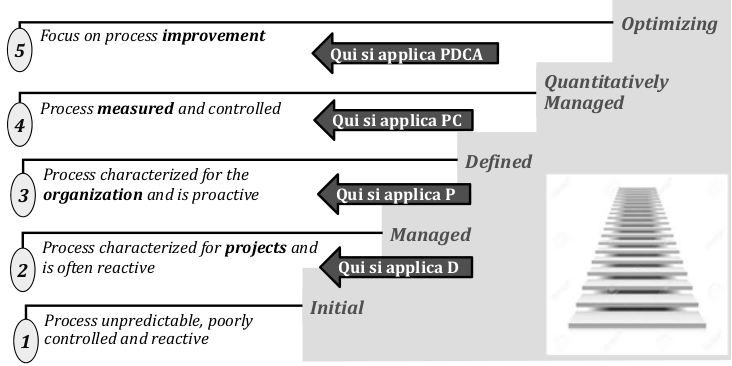
\includegraphics[width=0.9\textwidth]{img/maturity}
			\caption{I 5 livelli di maturità per la qualità di processo.}
		\end{figure}
		I livelli di maturità di \underline{\hyperref[cmmi]{CMMI}} mi aiutano a capire con quale intelligenza agisco.\\
		La maturità di prdotto valuta il grado di evoluzione del prodotto: quanto migliora in seguito alle prove, quanto diminuisce la densità dei difetti, quanto può costare la scoperta del prossimo difetto.


		\subsection{METRICA} \index{Metrica} \label{metrica}
		Integrale degli usi o utenti nel tempo.\\

		La \textit{Metrica Software} comprende:
			\begin{itemize}
				\item \textit{SLOC} (= Source Lines Of Code): conta le linee, è quindi oggettivamente misurabile e dà limiti;
				\item \textit{Effort}: risorse umane misurate come giorni/persona.
				\item \textit{Testo}: perché il testo è facilmente offuscabile, quindi si usa "l'indice di nebbia"/leggibilità.
			\end{itemize}
		Dà il modo di classificare attributi di processo e ci aiuta a ragionare a monte del problema e non a valle. In questo modo si possono predire gli attributi che arriveranno (capire prima se il prodotto farà schifo). L'obiettivo è quello di identificare anomalie \textit{"the sooner the better"}. \\
		Associate alla \underline{\hyperref[qualita]{Qualità del Software}} c'è l'idea di \textit{assunzioni} sulle metriche: nostro modo di pensare al problema. \\
		Attenzione perché non sempre si può misurare ciò che vogliamo. Ci interessa misurare ciò che è tracciabile di quello che vogliamo sapere (esempio dell'analisi del sangue: voglio sapere una cosa di alto livello non misurabile, tramite dati del mio sangue che sono misurabili). Importanti attributi sono: manutenibilità, affidabilità, \underline{\hyperref[portabilita]{portabilità}} e usabilità.\\
		%26 febbraio 2019 - Misurazione del software - Metodi e obiettivi di quantificazione
		%slide 16/25
		Il problema delle metriche SW è che il software è immateriale, difficile da misurare e le tecnologie SW cambiano rapidamente. \\
		%slide 17/25
		Metriche di progettazione:
		\begin{itemize}
			\item Grado di coesione
			\item Grado di accoppiamento: questo se alto è dannoso perchè la modifica in uno crea danni sull'altro.
			\item Complessità strutturale: dipendenza da fuori (metodo con 30 parametri). Funzione del fan-out (di una porta logica è il numero di porte logiche che possono essere collegate alla sua uscita).
			\item Complessità del flusso dati: funzione del numero di parametri in ingresso e in uscita.
			\item Complessità del sistema: funzione di complessità strutturale e complessità del flusso dati.
		\end{itemize}
		La \textit{complessità ciclomatica} ci interessa perchè più cammini ho, più test devo fare.


		\subsection{MISTAKE}	\index{Mistake}	\label{mistake}
		Ha a che vedere con la gerarchia di problemi nei \underline{\hyperref[test]{test}}. \\
		Ci siamo sbagliati noi nel produrre qualcosa che, se utilizzato  nel SW, causerà errore. Questo è quindi a monte di tutta la gerarchia.

		%26 febbraio 2019 - Misurazione del software - Metodi e obiettivi di quantificazione
		\subsection{MISURA}	\index{Misura} \label{misura}
		La misura assegna un valore quantitativo a un'entità per caratterizzarne un attributo specifico. \\
		\textbf{Obiettivo}: rendere oggettivi i risultati delle valutazioni effettuate (perchè siamo interessati in qualcosa di osservabile che ci aiuti a capire come siamo messi).
		Quest'oggettività implica:
		\begin{itemize}
			\item Ripetibilità
			\item Confrontabilità
			\item Confidenza
		\end{itemize}
		Nei limiti dell'approssimazione e della possibilità di astrazione. \\
		\textbf{Misura di realtà} è diverso da \textbf{indicatore}.
		La misura di realtà è per esempio il metro (per l'altezza).
		Gli indicatori invece ci servono per un confronto, mi suggerisoco qualcosa, ma sono solo degli indicatori. Non danno delle verità. \\
		Un giudizio di valutazione si forma con: %slide 7/25
		\begin{itemize}
			\item \textbf{Serie storica}: diagramma che ci dice l'andamento (esempio della polizia Svizzera che mette la multa). Dà delle tendenze nel tempo che sono molto utili.
			\item \textbf{Cruscotto}: alimentato in push, ovvero sempre valido, aggiornato e sempre a nostra disposizione. Ci deve dare informazioni.
		\end{itemize}
		Una \underline{\hyperref[metrica]{metrica}} di riferimento per la misurazione del software è \underline{\hyperref[leadtime]{lead time}}.




		\subsection{MOCK}	\index{Mock}	\label{mock}
		I \textit{mock object} (simulati o mock object) sono degli oggetti simulati che riproducono il comportamento degli oggetti reali in modo controllato. Nella programmazione ad oggetti, un programmatore crea un oggetto mock per testare il comportamento di altri oggetti, reali, ma legati ad un oggetto inaccessibile o non implementato. Allora quest'ultimo verrà sostituito da un mock.


		\subsection{MODELLI DI SVILUPPO} \index{Modelli di sviluppo} \label{modelli}
		Il modello è una costruzione astratta che fa capire qual è il problema e dà strumenti per risolverlo. È un riferimento ideale ad una cosa concreta, quindi astrazione non eseguibile, ma che mi definisce le proprietà. Date le diverse transizioni previste tra gli stati di un ciclo di vita e diverse regole di attivazione, esistono diversi tipi di modelli.
		%Flipped Classroom 6 dicembre
		I modelli, per essere tali, sono tutti "buoni". Semplicemente alcuni sono più adatti a certe esigenze rispetto ad altri.
		\begin{itemize}
			\item \textbf{A cosa serve}:
			Tre cose hanno fortissima influenza sulla scelta da fare:
			\begin{itemize}
				\item obiettivi;
				\item rischi;
				\item vincoli;
			\end{itemize}
			Serve a perseguire gli obiettivi cercando di rispettare i vincoli e mitigando i rischi.
			\item \textbf{Di cosa è fatto}:
			Il modello di sviluppo è legato al progetto da portare a termine e il progetto determina i processi. Quindi i processi hanno a che vedere con il modello di sviluppo. C'è un importante ordine di attività. Chi decide quali sono i \textit{gate} (momento in cui si termina un'attività e si passa a quella successiva) siamo noi, ovvero il fornitore, in base a quali obiettivi raggiungere nel tempo. Le milestone coincidono con i nostri gate. Le milestone c'entrano infatti sia con obiettivi, che con rischi e vincoli. \\
			Per dare elementi di mitigazione ai rischi ho la \underline{\hyperref[technologybaseline]{Technology Baseline}}. [Quante milestone ho lo decide il fornitore. La baseline sono le evidenze che porto per aprire i gate. Prima vengono le milestone e poi le baseline.] \\
			Il \underline{\hyperref[semat]{SEMAT}} mi dà l'essenza che sta alla radice di ogni modello di sviluppo. Dal SEMAT riesco a capire quali milestone adottare nel mio piano. E tra quelle che posso scegliere, le milestone che scelgo devono essere una confluenza di quelle più specializzate (ricordare le cards). Ho tante baseline quanti "lucchetti"(milestone) da aprire.
			\item \textbf{Come lo si attiva}: individuando le attività riconoscibili dalle baseline che ho scelto mettendole nel tempo disponibile e assegnandole.
		\end{itemize}

			\subsubsection{Sequenziale (o a cascata)} \index{Modello sequenziale} \label{msequenziale}
			\textbf{In breve}: ha rigide fasi sequenziali. \\
			 Tutto deve essere ripetibile (quindi anche migliorabile) e lineare (successioni di \underline{\hyperref[fase]{fasi}}), ma non ammette un ritorno a fasi precedenti. Adotta quindi una strategia in cui si continua o al più ci si ferma. Si prosegue solo se l'azione viene considerata buona (quindi documentata prima). I suoi prodotti sono principalmente \textit{documenti}. Ogni fase è caratterizzata da pre e post condizioni (di ingresso le prime e di uscita le seconde) e viene definita in termini di responsabilità e ruoli coinvolti. Dato che le fasi sono durate temporali, devono essere distinte e non sovrapposte nel tempo, dato che presentano delle dipendenze causali tra loro. Lo schema per il modello a cascata prevede in ordine: \underline{\hyperref[analisideirequisiti]{Analisi}} - \underline{\hyperref[progettazione]{Progettazione}} - \underline{\hyperref[realizzazione]{Realizzazione}} - \underline{\hyperref[manutenzione]{Manutenzione}}.  \\
			 \textbf{Difetto}: è totalmente rigido quindi ha bisogno di correttivi (come i \underline{\hyperref[prototipo]{prototipi}}).

			 \begin{figure}[H]
			 	\centering
			 	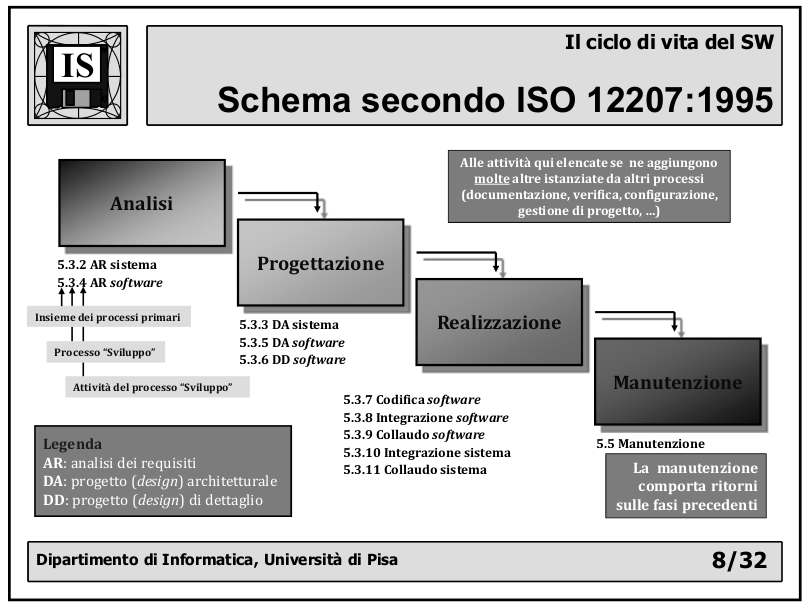
\includegraphics[width=0.8\textwidth]{img/cascata}
			 	\caption{Schema del modello a cascata secondo lo \underline{\hyperref[standard]{standard}} ISO 12207.}
			 \end{figure}

			\subsubsection{Incrementale} \index{Modello incrementale} \label{mincrementale}
			\textbf{In breve}: realizzazione in più passi, prevede rilasci multipli e successivi, ciascuno realizza un incremento di funzionalità. \\
			Dato che spesso non conviene posticipare l'integrazione di tutte le parti del sistema, risulta migliore l'\underline{\hyperref[integrazione]{integrazione continua}} di piccole parti. Sceglie un ordine di sviluppo che prepari il passaggio successivo motivo per cui ci vuole un modo strategico per capire come muoversi. I primi incrementi possono essere frutto di prototipazione,
			aiutando a fissare meglio i requisiti per gli incrementi successivi, ma i primi incrementi puntano a soddisfare i requisiti più importanti sul piano strategico così essi diventano presto chiari e stabili e quelli meno importanti si possono armonizzare al sistema. Ogni incremento riduce quindi il rischio di fallimento. Analisi e progettazione architetturale non vengono ripetute, dato che l'architettura del sistema è ben identificata e fissata dall'inizio, invece la realizzazione è incrementale (al momento della validazione può avvenire un ritorno).

			\begin{figure}[H]
				\centering
				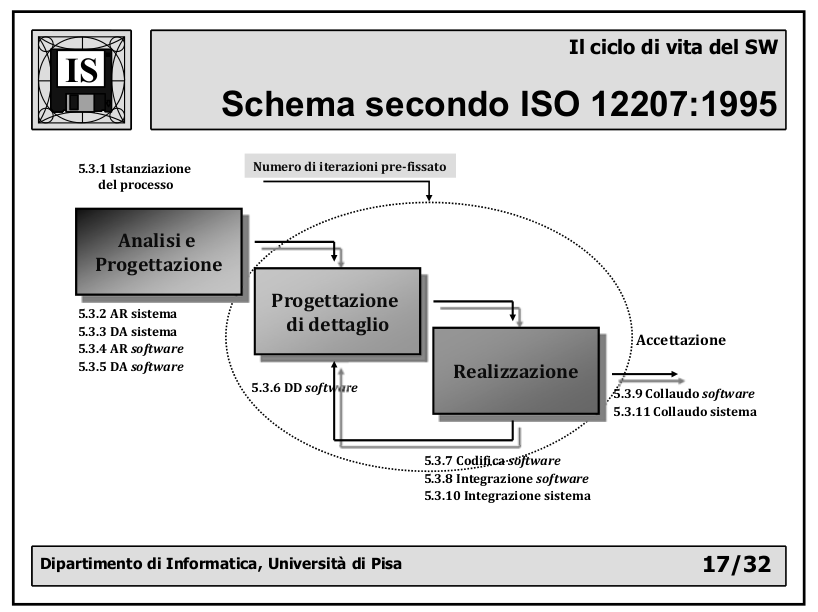
\includegraphics[width=0.8\textwidth]{img/incrementale}
				\caption{Schema del modello incrementale secondo lo \underline{\hyperref[standard]{standard}} ISO 12207.}
			\end{figure}

			\subsubsection{Iterativo} \index{Modello iterativo} \label{miterativo}
			\textbf{In breve}: ha ripetute iterazioni interne. \\
			Questo tipo di modello è applicabile a qualunque modello di ciclo di vita; consente infatti maggior capacità di adattamento. Il problema è che può andare incontro al rischio di non convergenza perché ogni iterazione comporta un ritorno all'indietro nella direzione opposta all'avanzamento del tempo. In generale conviene quindi decomporre la realizzazione del sistema in parti più piccole trattando prima le parti più critiche (magari quelle i cui requisiti vanno maggiormente chiariti).

			\subsubsection{A evoluzioni successive} \index{Modello a evoluzioni successive}
			\textbf{In breve}: comporta il riattraversamento di più stati di ciclo di vita. \\
			 \underline{\hyperref[prodotto]{Prodotto}} che evolve come conseguenza di una \underline{\hyperref[manutenzione]{manutenzione}}. Aiuta a rispondere a bisogni non inizialmente preventivabili. Inizialmente viene fatta un'analisi preliminare che identifica i requisiti e definisce l'architettura di massima e pianifica i passi di analisi. Dopodiché avviene l'analisi e realizzazione di una singola evoluzione (per raffinamento dell'analisi iniziale o per progettazione-codifica-prove-integrazione). Infine c'è il rilascio di versioni che man mano saranno sempre più complete. Ogni fase ammette iterazioni multiple e parallele.

			 \begin{figure}[H]
			 	\centering
			 	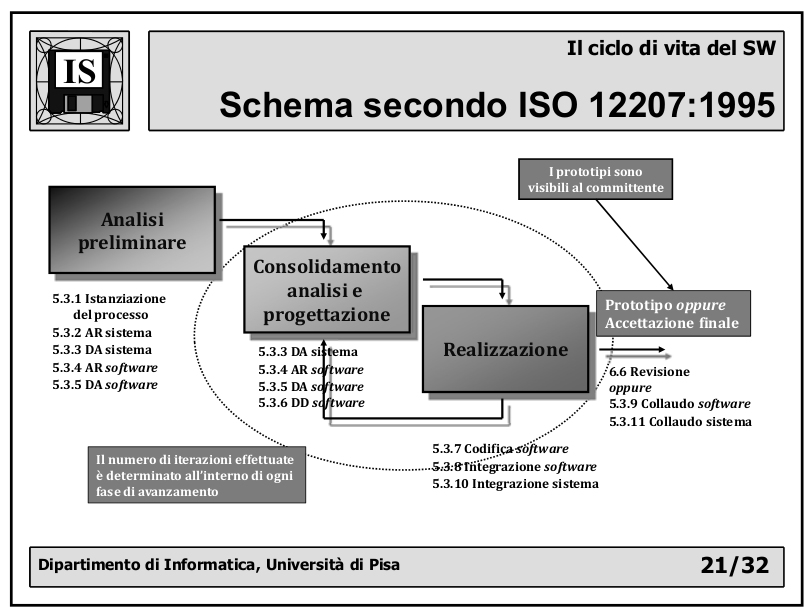
\includegraphics[width=0.8\textwidth]{img/evoluzione}
			 	\caption{Schema del modello evolutivo secondo lo \underline{\hyperref[standard]{standard}} ISO 12207.}
			 \end{figure}

			\subsubsection{Per componenti} \index{Modello per componenti}
			\textbf{In breve}: è orientato a massimizzare il riuso di software. \\
			 Decomposto in parti già esistenti e funzionanti, riusabili. L'analisi dei requisiti viene in seguito rivisitata in base alle possibilità di riuso.

			\begin{figure}[H]
				\centering
				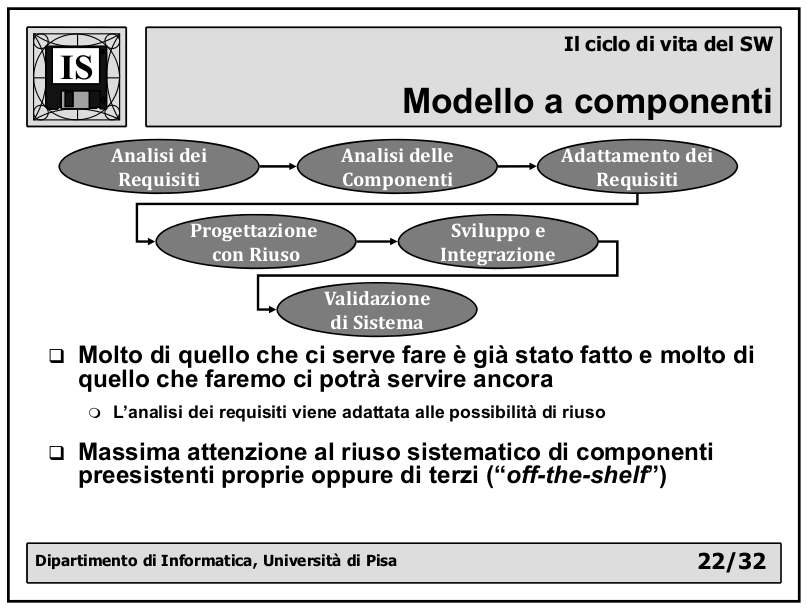
\includegraphics[width=0.8\textwidth]{img/acomponenti}
				\caption{Schema del modello a componenti secondo lo \underline{\hyperref[standard]{standard}} ISO 12207.}
			\end{figure}

			\paragraph{Il riuso}
			Dal Sommerville sappiamo del \textbf{riuso} che: \\
			Le unità software riusate possono avere diversa dimensione, per esempio:
			\begin{itemize}
				\item \textbf{System reuse}: un intero sistema (che può essere composto da più applicazioni) può essere riusato come parte di un sistema di tanti sistemi
				\item \textbf{Application reuse}: un'applicazione può essere riusata incorporandola in altri sistemi senza fare cambiamenti, oppure configurando l'applicazione per diversi customers
				\item \textbf{Component reuse}: componenti di un'applicazione (da sotto-sistemi a singoli oggetti) possono essere riusate. Per esempio, un sistema di sviluppo che fa pattern-matching, che fa parte di in un sistema di text-processing, può essere riusato in un sistema di gestione di database. Le componenti possono risiedere in un cloud o in server privati e possono essere accessibili tramite Application Programming Interface (API).
				\item \textbf{Object and function reuse}: componenti software che implementano una singola funzione o una classe oggetto possono essere riusate. Molte librerie di funzioni e classi sono liberamente disponibili. Si riusano classi e funzioni in queste librerie collegandole con lo sviluppo di nuovo codice.
			\end{itemize}
			A volte i sistemi o componenti sono così specifici che è molto costoso modificarli per una nuova situazione. Quindi, più che riusare il codice, è possibile riusare le idee che stanno alla base del software. Questo è chiamato \textbf{concept reuse} e tratta per esempio di riusare un way of working o un algoritmo e approcci quali i design patterns. \\
			I benefici del riuso sono:
			\begin{itemize}
				\item Costo complessivo di sviluppo più basso, perché meno componenti software devono essere progettate, implementate e validate
				\item Sviluppo accelerato
				\item Aumento di affidabilità, perchè software che è stato provato e testato in altri sistemi funzionanti è più affidabile di un nuovo software. I suoi difetti di progettazione e implementazione dovrebbero già esser stati trovati e sistemati.
				\item  Ridotto rischio di processo, vero specialmente per grandi componenti software riusate come sottosistemi. È un fattore importante per il Project Manager perché riduce il margine di errore nella stima dei costi di un progetto.
				\item Conformità con gli standard, perché alcuni standard, come gli interface standard, possono essere implementati come set di componenti riusabili
			\end{itemize}
			Ci sono però anche delle difficoltà legate al riuso come:
			\begin{itemize}
				\item Costo associato al capire se una componente è adatta al riuso per una particolare situazione o meno. È un costo aggiuntivo che potrebbe essere così elevato che potrebbe non abbassare il costo complessivo di sviluppo
				\item Creare, mantenere e usare la componente di una libreria, perché può essere oneroso
				\item Maggiori costi di manutenzione, perché se il codice sorgente della componente riusate non è disponibile, gli elementi riusati del sistema potrebbero diventare incompatibili con i cambiamenti fatti al sistema.
				\item Mancanza di strumenti di supporto, perché alcuni tools non supportano lo sviluppo con riuso.
				\item "Not-invented-here" syndrome, ovvero il fatto che alcuni software engineers preferiscono riscrivere componenti perchè credono di poterle migliorare
			\end{itemize}
			Fattori da considerare quando si sta pianificando il riuso:
			\begin{itemize}
				\item \textbf{The development schedule for the software}: se il software deve essere sviluppato velocemente, bisognerebbe riusare completamente un sistema piuttosto che una componente singola.
				\item \textbf{The expected software lifetime}: se si pensa ad un sistema con ciclo di vita lungo, bisognerebbe concentrarsi sulla manutenibilità del sistema. In questo caso si mira a riusare sistemi e componenti open-source più sicuri.
				\item \textbf{The background, skills and experience of the development team}: la cosa migliore è focalizzarsi nel riuso di aree in cui il team ha esperienza
				\item \textbf{The criticality of the software and its non-functional requirements}: per un sistema che deve essere certificato da un regolatore esterno, bisognerebbe creare una parte di sicurezza, ma questo è difficile se non si ha accesso al codice sorgente. Per esempio, se il software ha dei requisiti stringenti potrebbe risultare impossibile usare strategie quali il model-driven engineering (MDE).
				\item \textbf{The application domain}: in molti domini applicativi, come sistemi industriali e d'informazione medica, ci sono prodotti generici che possono essere riusati in una situazione locale. Qui fare riuso è spesso conveniente.
				\item \textbf{The platform on which the system will run}: come i .NET sono specifici delle piattaforme Microsoft, esistono sistemi di applicazioni generici che sono specifici di una certa piattaforma. Si è quindi in grado di riusare solo se il nostro sistema è progettato per la stessa piattaforma.
			\end{itemize}

		 	Per quel che riguarda i framework, Schimdt sostiene che il framework è: \textit{an integrated set of software artifacts (such as classes, objects and components) that collaborate to provide a reusable architecture for a family of related applications}. I frameworks forniscono supporto per caratteristiche generiche che possono essere usate in tutte le applicazioni di tipo simile. \\
		 	Quando una compagnia deve supportare un numero di sistemi simili ma non identici, uno degli approcci di riuso più efficaci è creare una \textit{software product line}. Una \textit{software product line} è un set di applicazioni con un'architettura comune e componenti condivise in cui ogni applicazione è specializzata per riflettere specifici requisiti del cliente.  Generalmente un'applicazione base include:
		 	\begin{itemize}
		 		\item \textbf{Core components}: forniscono un'infrastruttura di supporto e di solito non vengono modificate quando viene sviluppata una nuova istanza della \textit{software product line}.
		 		\item \textbf{Configurable application components}: possono essere modificate e configurate per specializzare una nuova applicazione.
		 		\item \textbf{Specialized application components}: specifiche del dominio, alcune o tutte possono essere rimpiazzare quando una nuova istanza della \textit{software product line} viene creata.
		 	\end{itemize}

	 	 	\paragraph{CBSE}
	 	 	Le componenti sono ad un livello di astrazione più alto degli oggetti e sono definite dalle loro interfacce. Sono solitamente più grandi degli oggetti singoli e tutti i dettagli implementativi sono nascosti alle altre componenti. \\
	 		\textit{Component-based software engineering} è il processo di definizione, implementazione e integrazione o composizione di queste componenti scarsamente accoppiate e indipendenti nei sistemi.  \\
	 		Le caratteristiche essenziali un una componente usate nel CBSE (\textit{Component-based software engineering}):
	 		\begin{itemize}
	 			\item \textbf{Composable}
	 			\item \textbf{Deployable}
	 			\item \textbf{Documented}
	 			\item \textbf{Independent}
	 			\item \textbf{Standardized}
	 		\end{itemize}
 			Un modo utile di vedere una componente è vederla come un fornitore di uno o più servizi:
 			\begin{itemize}
 				\item La \textbf{componente} è un'entità eseguibile indipendente che viene definita dalla sua interfaccia. Non c'è bisogno di saperne il codice sorgente per usarla.
 				\item I \textit{servizi} offerti da una componente sono resi disponibili attraverso un'interfaccia e tutte le interazioni avvengono tramite quell'interfaccia. L'interfaccia della componente è espressa in termini di operazioni parametrizzate e il suo stato interno non è mai esposto.
 			\end{itemize}
 			Di base tutte le componenti hanno due interfacce collegate:

 			\begin{figure}[H]
 				\centering
 				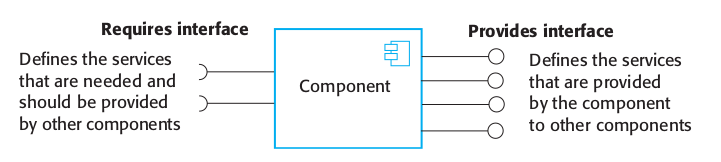
\includegraphics[width=0.8\textwidth]{img/interfaces}
 				\caption{Interfacce di una componente.}
 			\end{figure}

 			\begin{itemize}
 			 	\item La \textit{requires interface} specifica i servizi che le altre componenti del sistema devono fornire affinchè la componente funzioni correttamente. Se questi servizi non sono disponibili, la componente non funzionerà.
 			 	\item La \textit{provides interface} definisce i servizi forniti dalla componente. Quest'interfaccia è la componente API.
 			\end{itemize}

 			\paragraph{Component models}
 			Un \textit{component model} è una definizione di standard per l'implementazione, la documentazione e il deployment di componenti. Questi standard sono per gli sviluppatori delle componenti per assicurare che le componenti siano interoperabili. Per \textit{service components} il più importante modello a componenti è il Web Service model, mentre per le \textit{embedded components} sono ampiamenti usati i modelli Enterprise Java Beans(EJB) e Microsoft's .NET.

 			\begin{figure}[H]
 				\centering
 				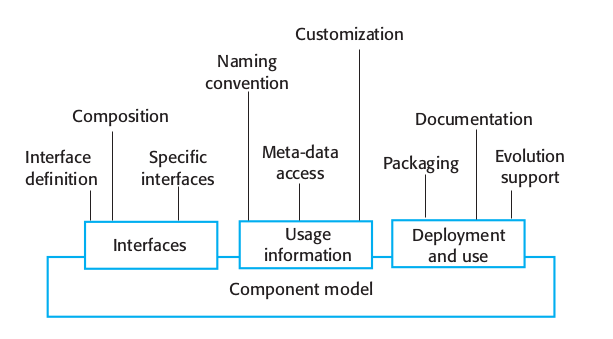
\includegraphics[width=0.8\textwidth]{img/componentmodel}
 				\caption{Elementi base di un component model.}
 			\end{figure}

 			\paragraph{CBSE processes}
 			I processi CBSE sono processi software che supportano la \textit{Component-Based Software Engineering}. Ne esistono di due tipi:
 			\begin{itemize}
 				\item \textbf{Development for reuse}: processo mirante allo sviluppo di componenti o servizi che saranno riusati in altre applicazioni. Generalmente coinvolge componenti generiche già esistenti.
 				\item \textbf{Development with reuse}: processo che sviluppa nuove applicazioni usando componenti e servizi esistenti.
 			\end{itemize}


			\subsubsection{Agile} \index{Modello agile}
			\textbf{In breve}: è altamente dinamico ed è fatto di brevi ciclo iterativi e incrementali. \\
			Basato su principi fortemente di reazione che sono:
				\begin{enumerate}
			 		\item \textit{Individuals and interactions over processes and tools}: l’eccessiva rigidità ostacola l’emergere del valore;
			 		\item \textit{Working sofware over comprehensive documentation}: la documentazione non sempre corrisponde a SW funzionante
			 		\item \textit{Customer collaboration over contract negotiation}: l’interazione con gli stakeholder va incentivata;
			 		\item \textit{Responding to change over following a plan}: la capacità di adattamento al cambiare delle situazioni;
			 	\end{enumerate}
		 	Si basa sull'idea di \textit{user story}, ovvero una funzionalità che è significativa per l'utente e che vuole nella realizzazione del software richiesto. Ogni \textit{user story} è definita un documento che descrive il problema, una sintesi delle conversazioni di discussione del problema con gli \underline{\hyperref[stakeholder]{stakeholder}} e la strategia da adottare per soddisfare il problema. Si prosegue suddividendo il lavoro in piccoli  \underline{\hyperref[incremento]{incrementi}} (che possono essere sviluppati anche indipendentemente) sviluppati in modo continuo e sequenziale dall'analisi all'integrazione. Gli \textit{obiettivi strategici} sono poter dimostrare costantemente al cliente quanto fatto e che l'intero  \underline{\hyperref[prodotto]{prodotto SW}} sia ben integrato e verificato.
		 	[NB: Non é molto buono. É assente la documentazione quindi é più un costo che un valore]

			\subsubsection{SCRUM}	\index{Modello SCRUM}	\label{scrum}
			\textbf{In breve}: è un tipo di Modello Agile ["mischia di rugby"]. \\
			È costituito da:
				\begin{itemize}
					\item \textbf{Product \underline{\hyperref[backlog]{backlog}}}: requisiti e funzionalità del prodotto;
					\item \textbf{Sprint}: fase operativa di sviluppo;
					\item \textbf{Sprint \underline{\hyperref[backlog]{backlog}}}: insieme di storie del prossimo sprint;
					\item \textbf{Sprint Planning}: pianificazione dello sprint;
					\item \textbf{Daily Scrum}: controllo giornaliero dell'avanzamento;
					\item \textbf{Sprint Review}: controllo prodotti dello sprint;
					\item \textbf{Sprint Retrospective}: controllo \underline{\hyperref[qualita]{qualità}} sullo sprint;
				\end{itemize}

			\subsubsection{A spirale} \index{Modello a spirale}
			(Complicato, non lo trattiamo). Va da un problema piccolo ad uno sempre più grande. Pensato per attività che non hanno una \underline{\hyperref[best]{best practice}} ben nota.


		\subsection{MODULI}	\index{Moduli}	\label{moduli}
		La più piccola entità progettuale che sia utile rappresentare.
